\documentclass{article}

%% Page Margins %%
\usepackage{geometry}
\geometry{
    top = 0.75in,
    bottom = 0.75in,
    right = 0.75in,
    left = 0.75in,
}

\usepackage{amsmath}
\usepackage{graphicx}
\usepackage{parskip}

\title{Assembly Project: Dr Mario (Solo)}

% TODO: Enter your name
\author{Yuchen Gao}

\begin{document}
\maketitle

\section{Instruction and Summary}

\begin{enumerate}

    \item Which milestones were implemented? 

    \begin{enumerate}

    \item Milestone 1
    \item Milestone 2
    \item Milestone 3
    \item Milestone 4
        \begin{enumerate}
        \item Easy Feature 1: Implemented gravity
        \item Easy Feature 2: Implemented gravity speed increment over time
        \item Easy Feature 4: Implemented Game Over and Retry
        \item Easy Feature 6: Implemented Pause when player presses the key p
        \end{enumerate}
    \item Milestone 5
        \begin{enumerate}
        \item Easy Feature 3: Implemented 3 different game mode
        \item Easy Feature 11: Implemented a preview of the next capsule
        \item Easy Feature 12: Augment the panel in Easy Feature 11 to display a preview of the next 4-5 capsules
        \item Easy Feature 8: Added an outline where the capsule will end up if you drop it
        \end{enumerate}
    \end{enumerate}
    

    \item How to view the game:
    
    
    % TODO: specify the pixes/unit, width and height of 
    %       your game, etc.  NOTE: list these details in
    %       the header of your breakout.asm file too!
    
    \begin{enumerate}

    \item Unit width in pixels:       2
    \item Unit height in pixels:      2
    \item Display width in pixels:    64
    \item Display height in pixels:   64
    \end{enumerate}

    

\begin{figure}[ht!]
    \centering
    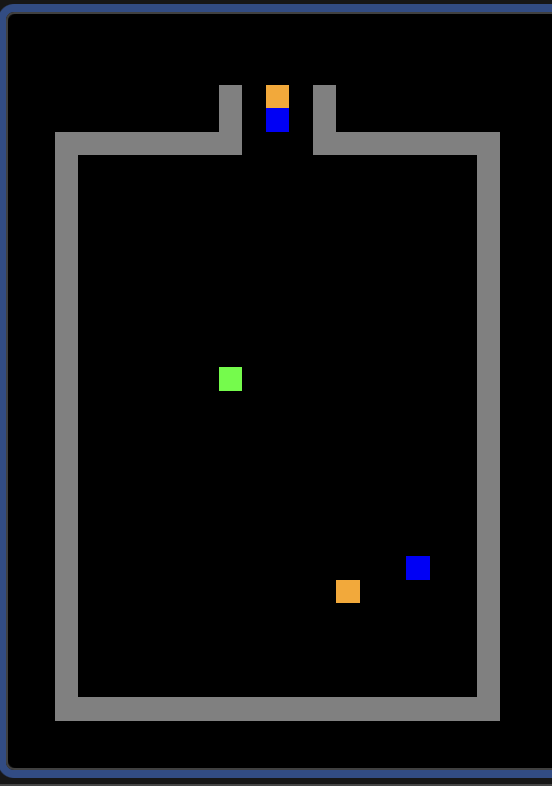
\includegraphics[width=0.3\textwidth]{Milestone1_with_viruses.png}
    \caption{Static Scene of the background of the game}
    \label{Instructions}
\end{figure}

\item Game Summary:
% TODO: Tell us a little about your game.
\begin{itemize}
\item I code the scene of the game in two different ways. The first time I hard coded everything. After attending the Lecture on draw\_rect, I realized that drawing the scene by calling the function draw\_rect would be much more efficient. So I cleaned up my code a bit by calling draw\_rect instead.
\item The way my game generate new capsule is by calling a random number generator that outputs 3 different numbers and then based on the number assign the color blue, green or orange. Repeat the process for the other of the capsule and it will generate a pseudo-random 2-halves capsule.
\end{itemize}

    
\end{enumerate}

\end{document}